%
% An Appendix
\chapter{Indoor Localization Experiment}
\label{appendix:shs_experiment}
\textbf{Apparatus}:

\emph{Hardware}:

\begin{itemize}
	\item
	3 Smartphones
	
	\begin{itemize}
		\tightlist
		\item
		Samsung j5 for video recording
		\item
		Iphone for backup orientation estimation and post processing time
		synchronization
		\item
		One Plus Nord for primary orientation estimation and ground truth
		activity recorder
	\end{itemize}
	\item
	1 apple smartwatch
	\item
	Shirt with two breast pockets
	\item
	Indoor test location
\end{itemize}

\emph{Software}:

\begin{itemize}
	\tightlist
	\item
	Iphone and apple watch app
	(\url{https://apps.apple.com/us/app/sensorlog/id388014573\#?platform=appleWatch})
	\item
	Android app for primary sensor recording
	(\url{https://play.google.com/store/apps/details?id=fr.inria.tyrex.senslogs\&hl=en\&gl=US}
	)
\end{itemize}

\textbf{Calibration}:

Calibrate primary estimation sensor (One Plus Nord) just before
experiment, and perform all calibration at the same location within test
location!

\begin{itemize}
	\item
	\emph{Magnetometer}:
	
	\begin{itemize}
		\tightlist
		\item
		Stand away from any clear magnetic disturbance 
		\item
		rotate the phone in as many orientations as possible, infinity sign
		is often used
	\end{itemize}
	\item
	\emph{Accelerometer}:
	
	\begin{itemize}
		\tightlist
		\item
		Rotate the phone slowly in as many orientations as possible in
		attempting to be in as many orientations as possible.
	\end{itemize}
	\item
	\emph{Gyroscope / Magnetic North / Noise}
	
	\begin{itemize}
		\item
		Lay the phone horizontally and start recording while stationary
	\end{itemize}
\end{itemize}

\textbf{Preparation}:

\begin{enumerate}
	\def\labelenumi{\arabic{enumi}.}
	\tightlist
	\item
	Calibrate One Plus Nord with the calibration method outlined above
	\item
	Determine with which hand you will hold the phone, strap the
	smartwatch to the other hand
	\item
	Ensure that all doors in test location are closed
	\item
	Define start location within test location and record it
\end{enumerate}

\textbf{Testing}:

For \emph{each test run} perform the following steps:

\begin{enumerate}
	\def\labelenumi{\arabic{enumi}.}
	\tightlist
	\item
	Go to start location
	\item
	Start sensor recording on smartwatch and iPhone
	\item
	place iPhone in one of the breast pockets of the shirt
	\item
	Start a video recording on the Samsung phone and place it in the other
	breast pocket, making sure that the lens is not covered and can see
	what is in front of the torso of the test subject, hence also what
	direction is being moved in.
	\item
	Start sensor recording on One Plus Nord, logging the uncalibrated
	accelerometer, gyroscope, and magnetometer. Also record the rotation
	vector that the phone records. This is shown in illustration 1.
	\item
	Walk around test location as naturally as possible, holding the One
	Plus Nord in front of you with the screen point up. Try and keep this
	phone orientation as best as possible.
	\item
	Walk to doors and open them using the arm that has the smartwatch on
	it. When touching a door handle click the button in the android app
	that records the time stamp as shown in illustration 2. Close the door
	behind you, so that it can potentially be opened again later.
	\item
	After walking for around 3 minutes, return to start location
	\item
	Stop recording of sensor and video on all devices
	\item
	export the data (film and sensor) from all 3 devices to the same
	folder, making it clear which trail it was
\end{enumerate}

\textbf{Pictures}:
\begin{figure}[H]
	\centering
	\begin{subfigure}[t]{.45\textwidth}
		\centering
		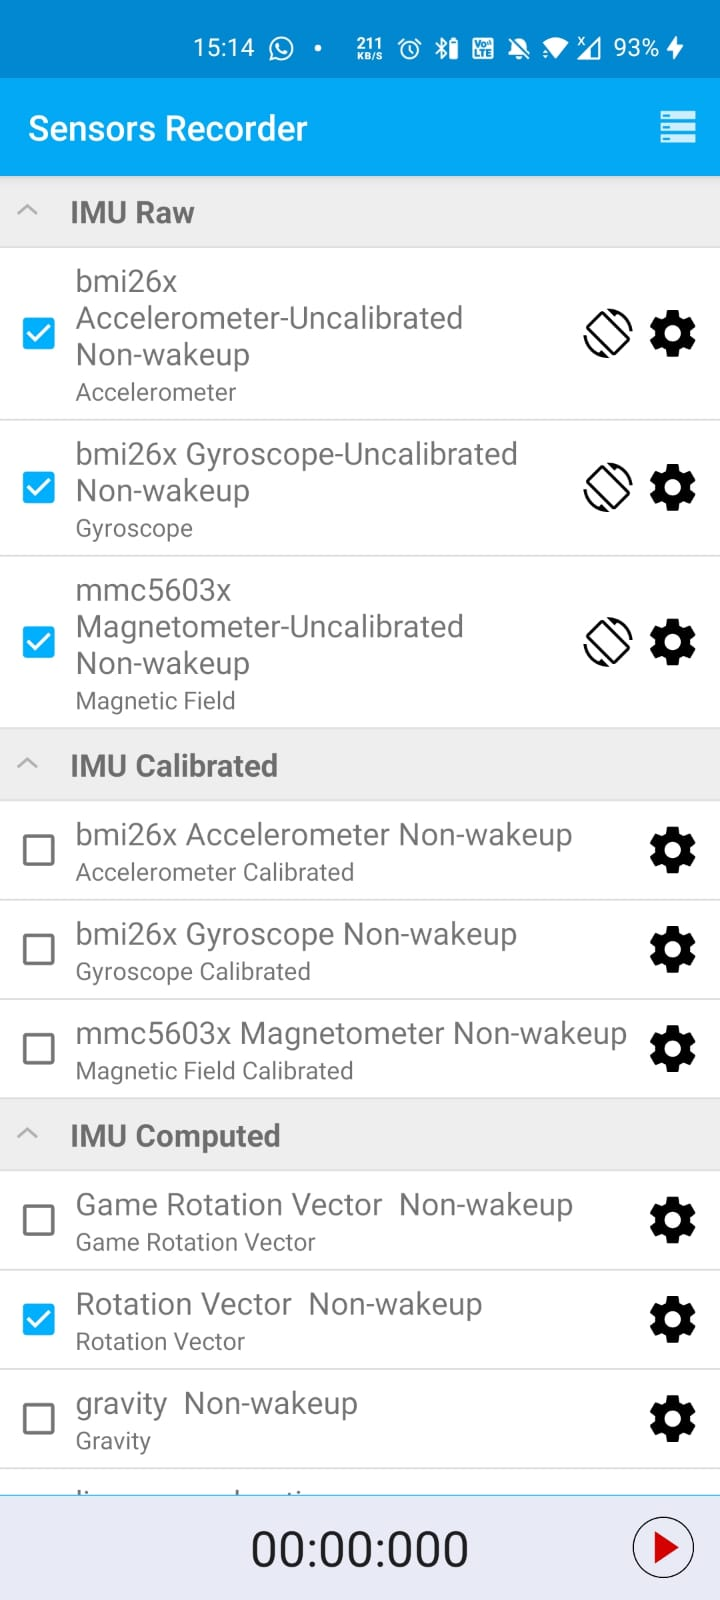
\includegraphics[width=0.6\linewidth]{images/recording_setting}
		\caption{Recording settings}
		\label{fig:recording_setting}
	\end{subfigure}
	\begin{subfigure}[t]{.45\textwidth}
		\centering
		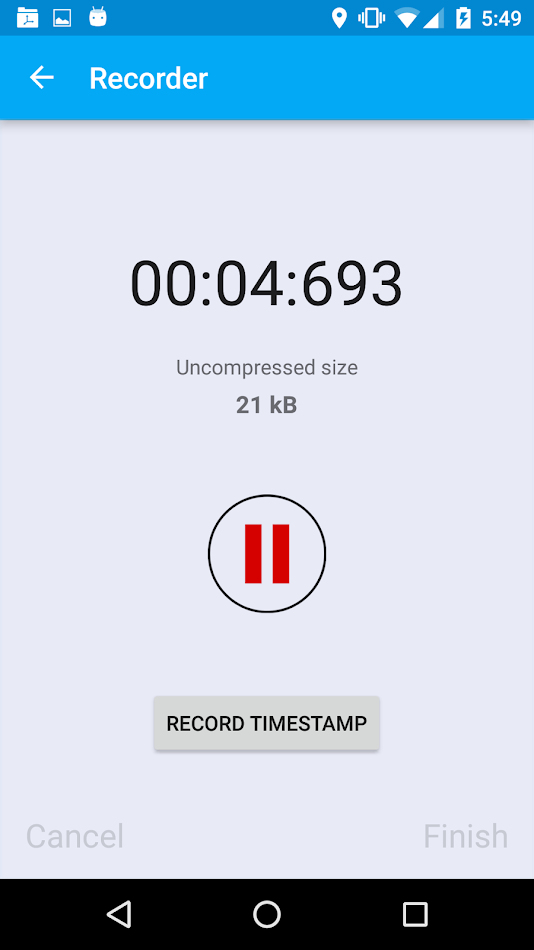
\includegraphics[width=0.7\linewidth]{images/recording_timestamp_button}
		\caption{Record timestamp button}
		\label{fig:recording_timestamp_button}
	\end{subfigure}
\caption{Indoor experiment android app configuration and button}
\end{figure}


\textbf{Postprocessing}

\begin{enumerate}
	\def\labelenumi{\arabic{enumi}.}
	\tightlist
	\item
	Calibrate walking around imu sensor data using calibration data
	\item
	Run calibrated walking around data through orientation estimation
	algorithm
	\item
	Compare result with orientation estimation made by the system and
	maybe even with the iphone 
	\item
	Determine steps and subsequent step length 
	\item
	Combine orientation information and step information to generate an
	estimated trajectory
	\item
	Use this estimated trajectory as input for the particle filter
	\item
	Using the video recording made during testing, manually indicate per
	step where on the blueprint you are. This will be used to determine
	the performance of the estimate of the SHS system. 
\end{enumerate}

\chapter{Indoor Experiment Results}

\section{SHS-PF parameter search}
\begin{figure}[H]
	\centering
	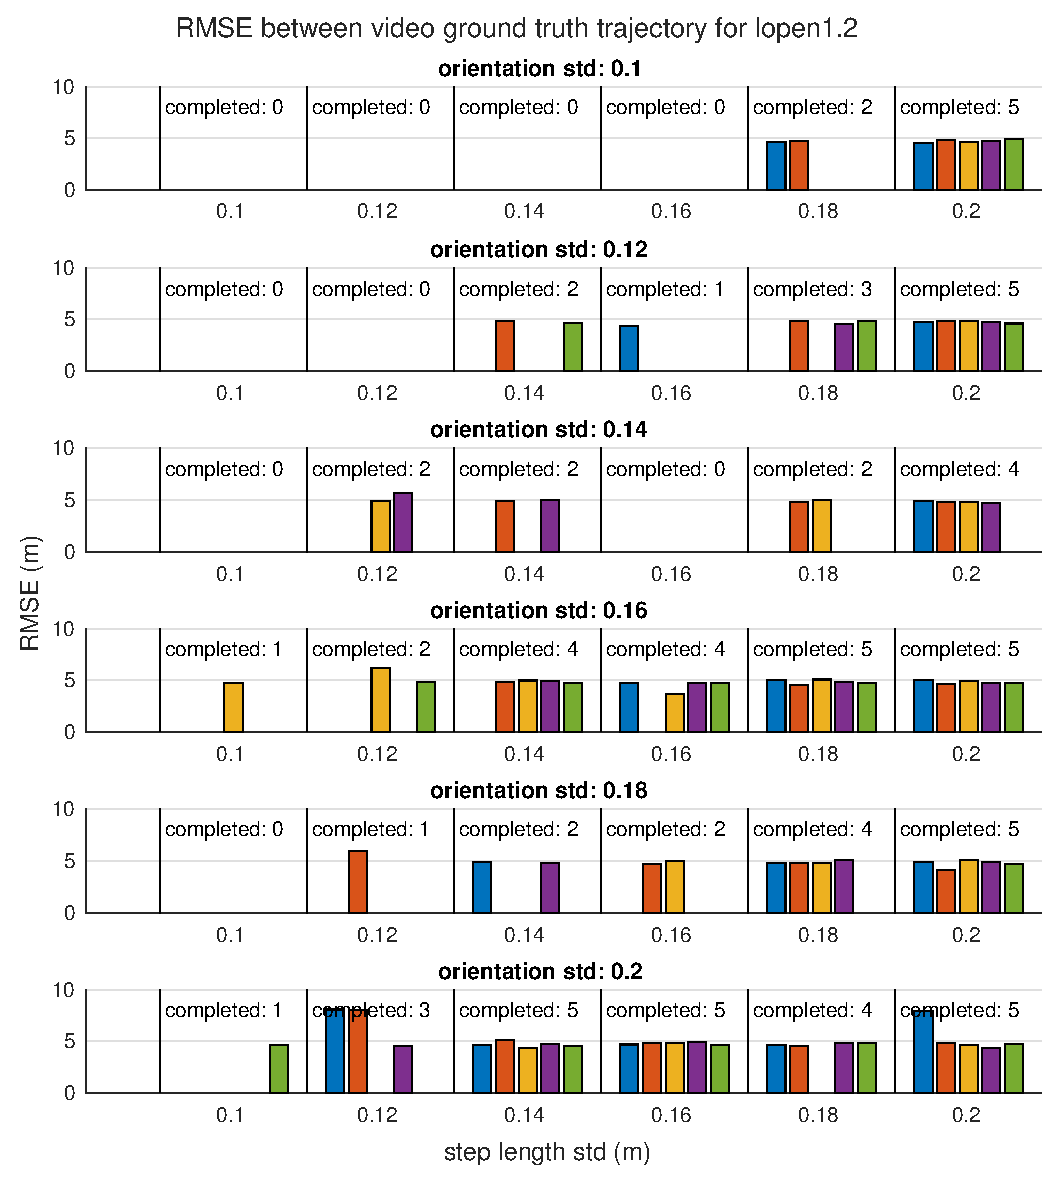
\includegraphics[width=0.7\linewidth]{images/20201107_1312_orientation_std_0_2}
	\caption{}
	\label{fig:202011071312orientationstd02}
\end{figure}
\begin{figure}[H]
	\centering
	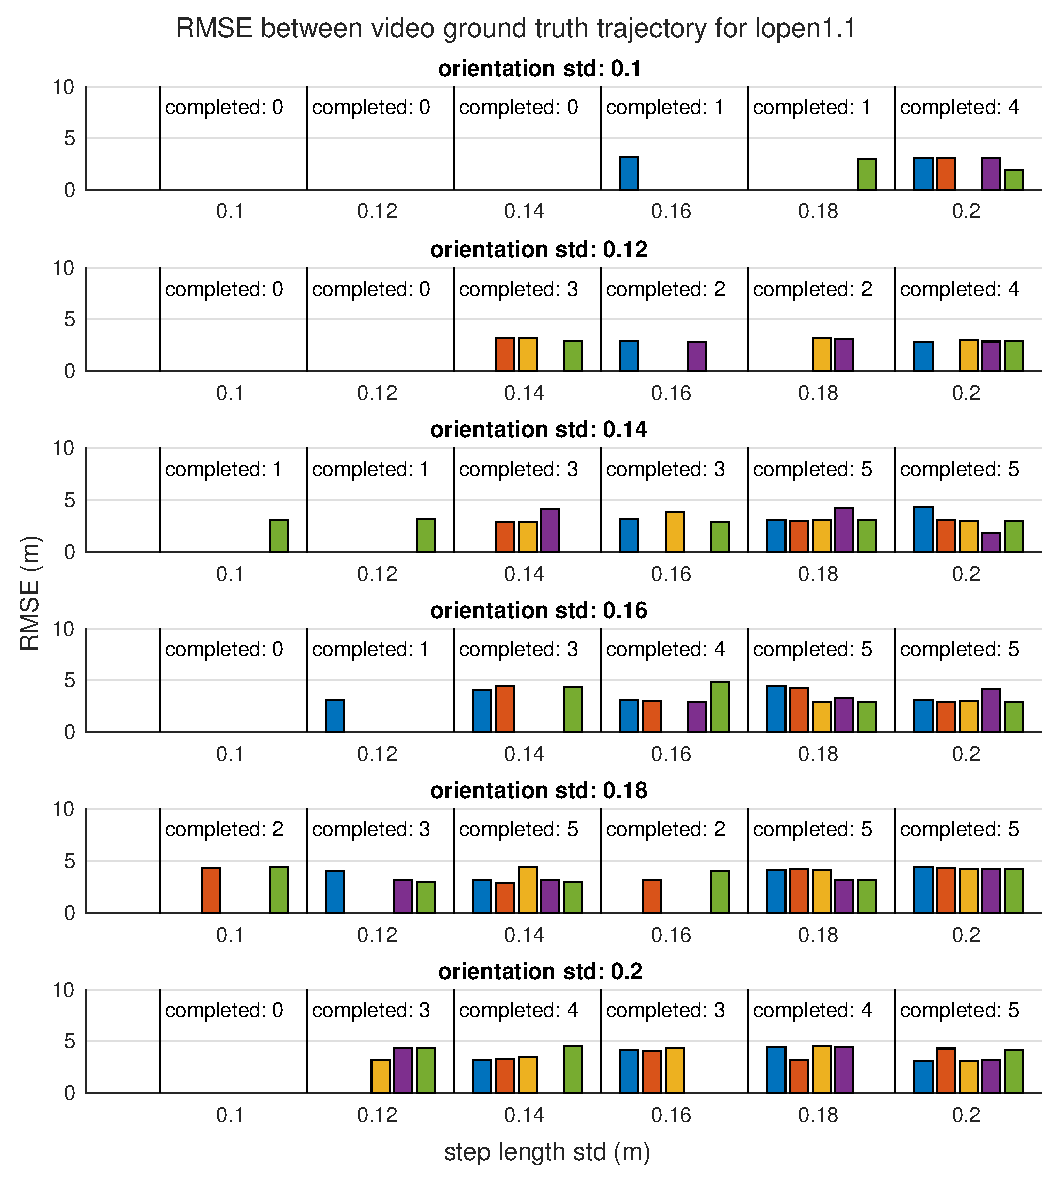
\includegraphics[width=0.7\linewidth]{images/20201107_1311_orientation_std_0_2}
	\caption{}
	\label{fig:202011071311orientationstd02}
\end{figure}

\section{SHS-PF estimator comparison}
\begin{figure}[H]
	\centering
	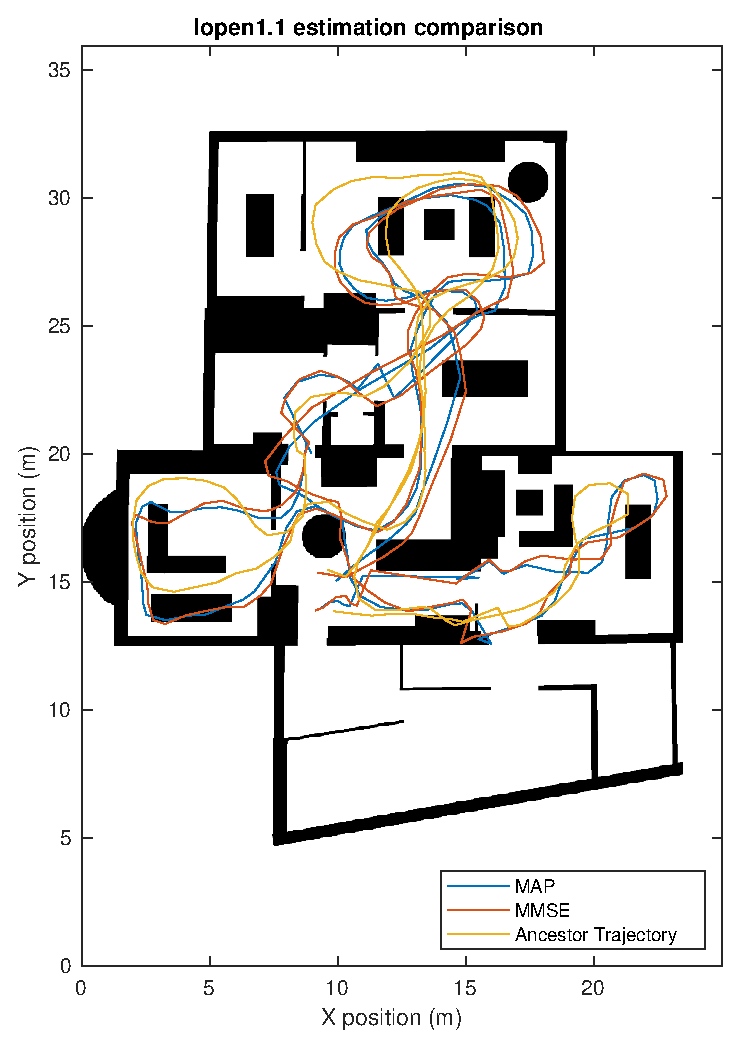
\includegraphics[width=0.5\linewidth]{images/20201108_1559_lopen1_1_estimation_comparison}
	\caption{}
	\label{fig:202011081559lopen11estimationcomparison}
\end{figure}
\begin{figure}[H]
	\centering
	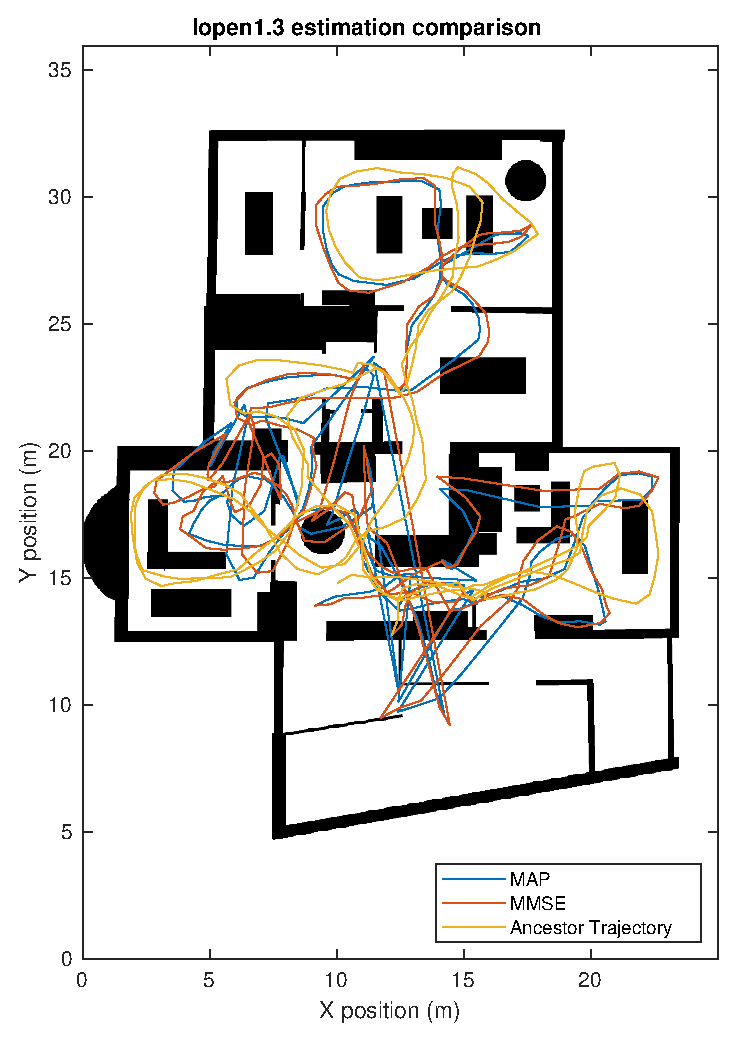
\includegraphics[width=0.5\linewidth]{images/20201108_1601_lopen1_3_estimation_comparison}
	\caption{}
	\label{fig:202011081601lopen13estimationcomparison}
\end{figure}
\begin{figure}[H]
	\centering
	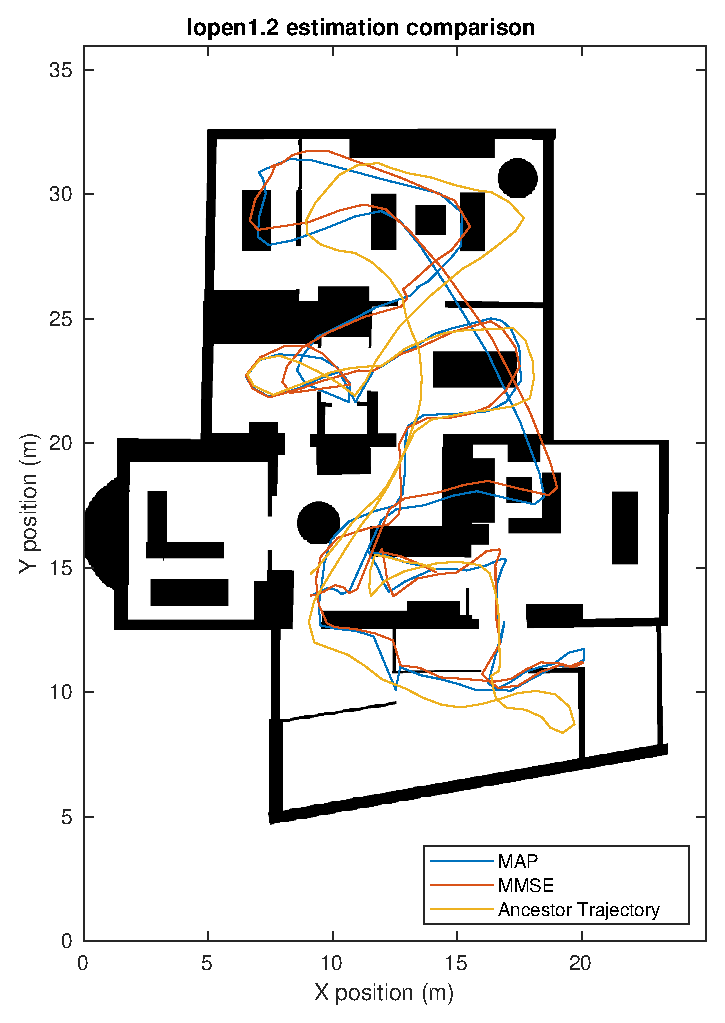
\includegraphics[width=0.5\linewidth]{images/20201108_1559_lopen1_2_estimation_comparison}
	\caption{}
	\label{fig:202011081559lopen12estimationcomparison}
\end{figure}




\section{SHS-PF performance}
\label{app:SHS-PF trials}
\begin{figure}[H]
	\centering
	\begin{subfigure}[t]{.45\textwidth}
	\centering
	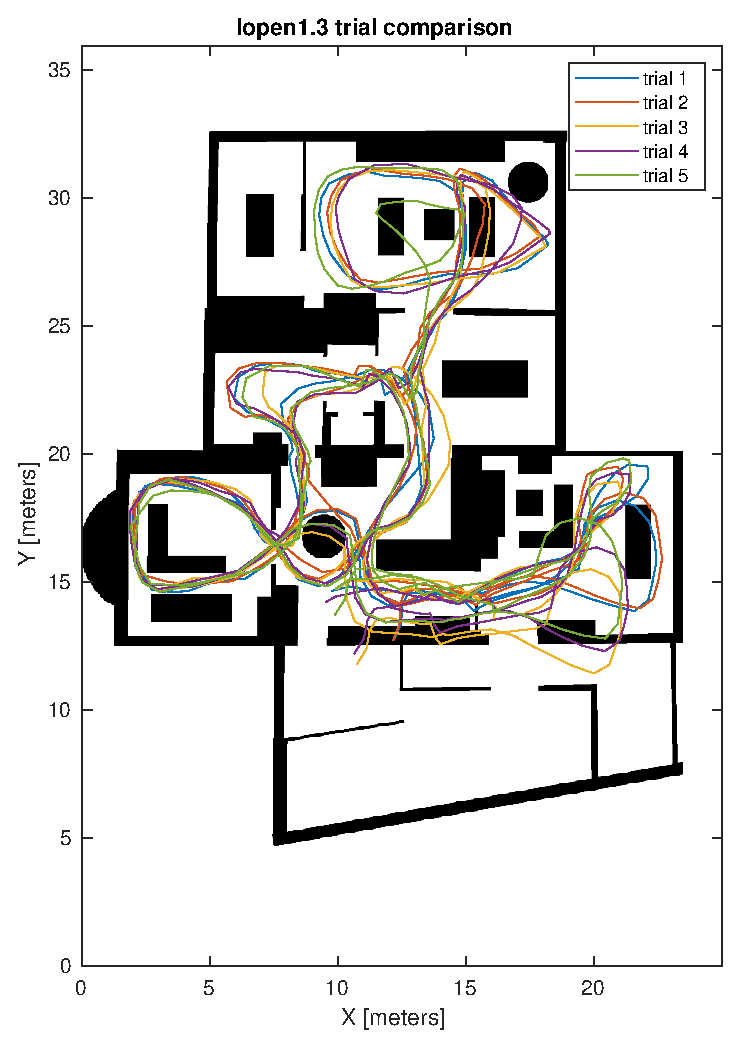
\includegraphics[width=\linewidth]{images/20201107_1142_trial_comparison_3}
	\caption{}
	\label{fig:202011071142trialcomparison3}
\end{subfigure}
\begin{subfigure}[t]{.45\textwidth}
	\centering
	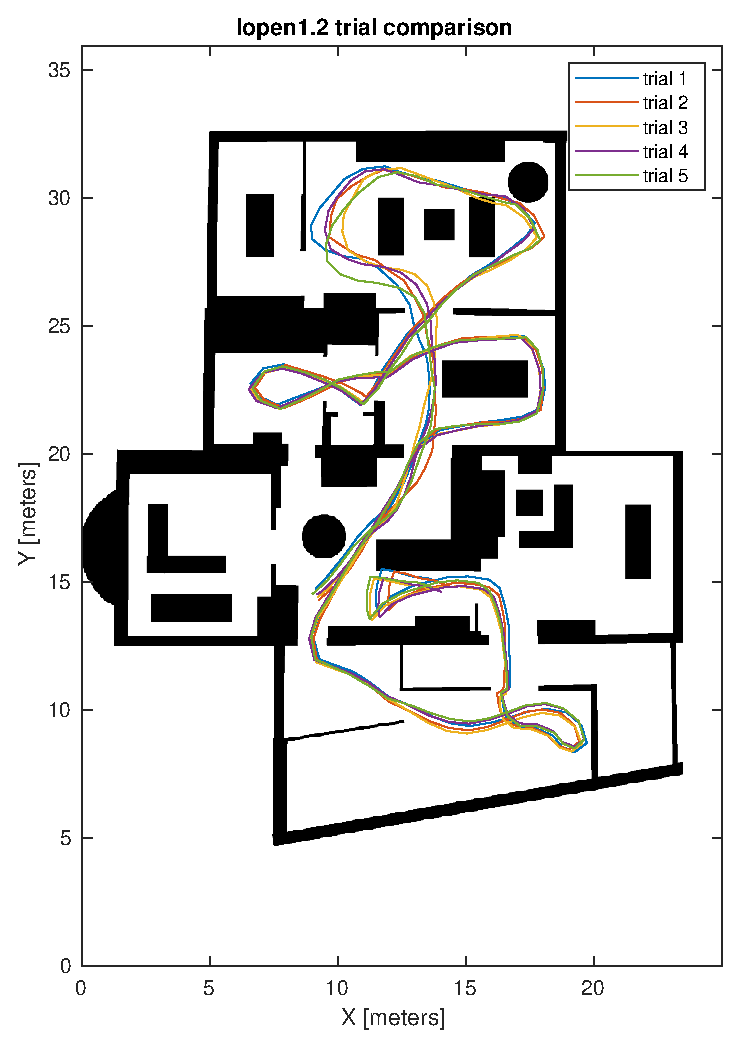
\includegraphics[width=\linewidth]{images/20201107_1142_trial_comparison_2}
	\caption{}
	\label{fig:202011071142trialcomparison2}
\end{subfigure}
\end{figure}

\begin{figure}
	\centering
	\begin{subfigure}[t]{.45\textwidth}
		\centering
		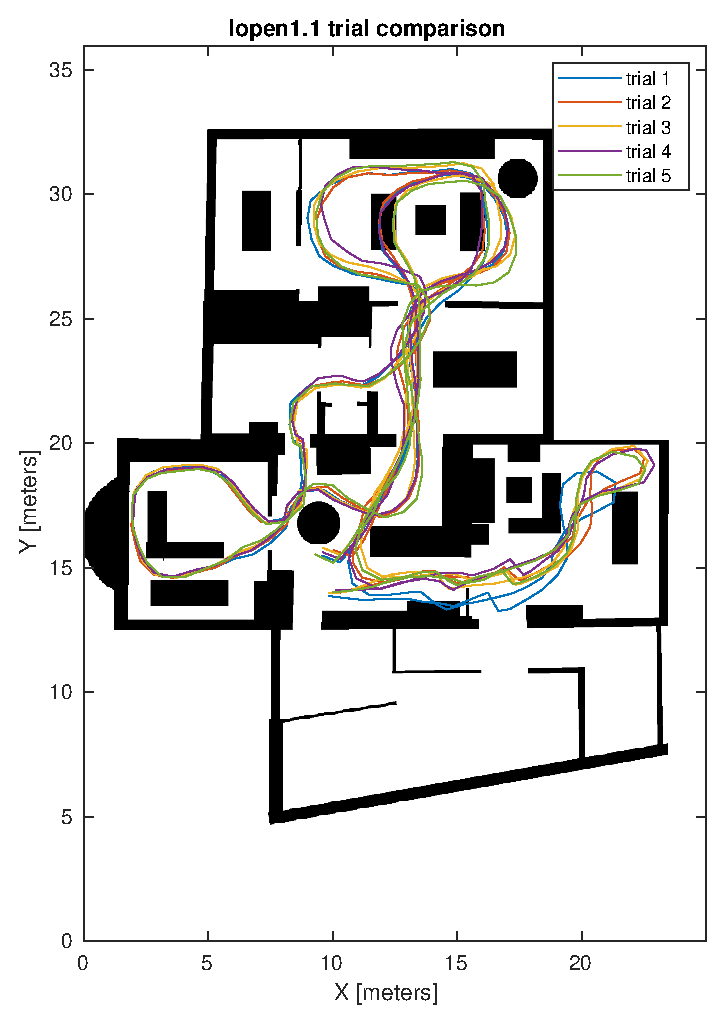
\includegraphics[width=\linewidth]{images/20201107_1142_trial_comparison_1}
		\caption{}
		\label{fig:202011071142trialcomparison1}
	\end{subfigure}
\end{figure}


